\chapter{Findings}
\label{cha:findings}
% Grading Criteria
% - Steps taken to arrive at the presented findings 
% - The research question is addressed
% - present findings
% - graphs and table support the main findings 
% - findings are presented without judgment

This section presents the findings of the papers introduced in \autoref{subsec:k_means_in_the_context_of_energy_saving_incentives}.
The differences and similarities are juxtaposed for both research questions.

% Wie möchte ich die Research Questions erklären?
% Es werden nicht die Fragen beantwortet, sondern vielmehr eine Hinführung zur Conclusion gegeben,
% Also nicht auf die Conclusion eingehen, sondern auf die Results der jeweiligen Paper
% - Zusammenhängend => Mehr ein Fließtext, der die Fragen mithilfe der Paper beantwortet
% - Jedes Ergebnis soll so erklärt werden, dass es in den jeweiligen Kontext hineinpasst
% - Dabei alles sauber labeln und möglichst viel zitieren
\section{Improving the Design of Energy-Saving Incentives}
\label{sec:improving_the_design_of_energy_saving_incentives}

TODO: Delete the paragraphs and summarize both findings in continuous text
\paragraph*{LIU-BDE:}


\begin{figure}
    \centering
    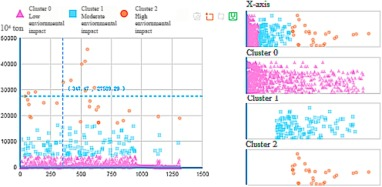
\includegraphics[width=0.8\textwidth]{figures/liu_assessmentOfIndustries/liu_environmentalPerformance.jpg}
    \caption{Multi-Industries Clustering Result based on the $SO_2$ Emission \cite{LIU-BDE}}
    \label{fig:multi_industries_clustering_result_environemental_performance}
\end{figure}

\begin{table}
    \centering
    \begin{tabular}{c|c|c|c|c}
        \texttt{Fields} & \texttt{Sum} & \texttt{Cluster 0} & \texttt{Cluster 1} & \texttt{Cluster 2} \\
        \hline
        Chemical Industry & 144 & 138 & 0 & 6 \\
        Coal Mining and Washing Industry & 60 & 54 & 4 & 2 \\
        Textile Industry & 49 & 49 & 0 & 0 \\
        Paper Products Industry & 47 & 42 & 0 & 5 \\
    \end{tabular}
    \caption{Snippet of the Multi-Industries Clustering Results based on the $SO_2$ Emission \cite{LIU-BDE}}
    \label{tab:multi_industries_clustering_results_based_on_the_so2_emission}
\end{table}

\paragraph*{MAL-EMD:}


\begin{figure}
    \centering
    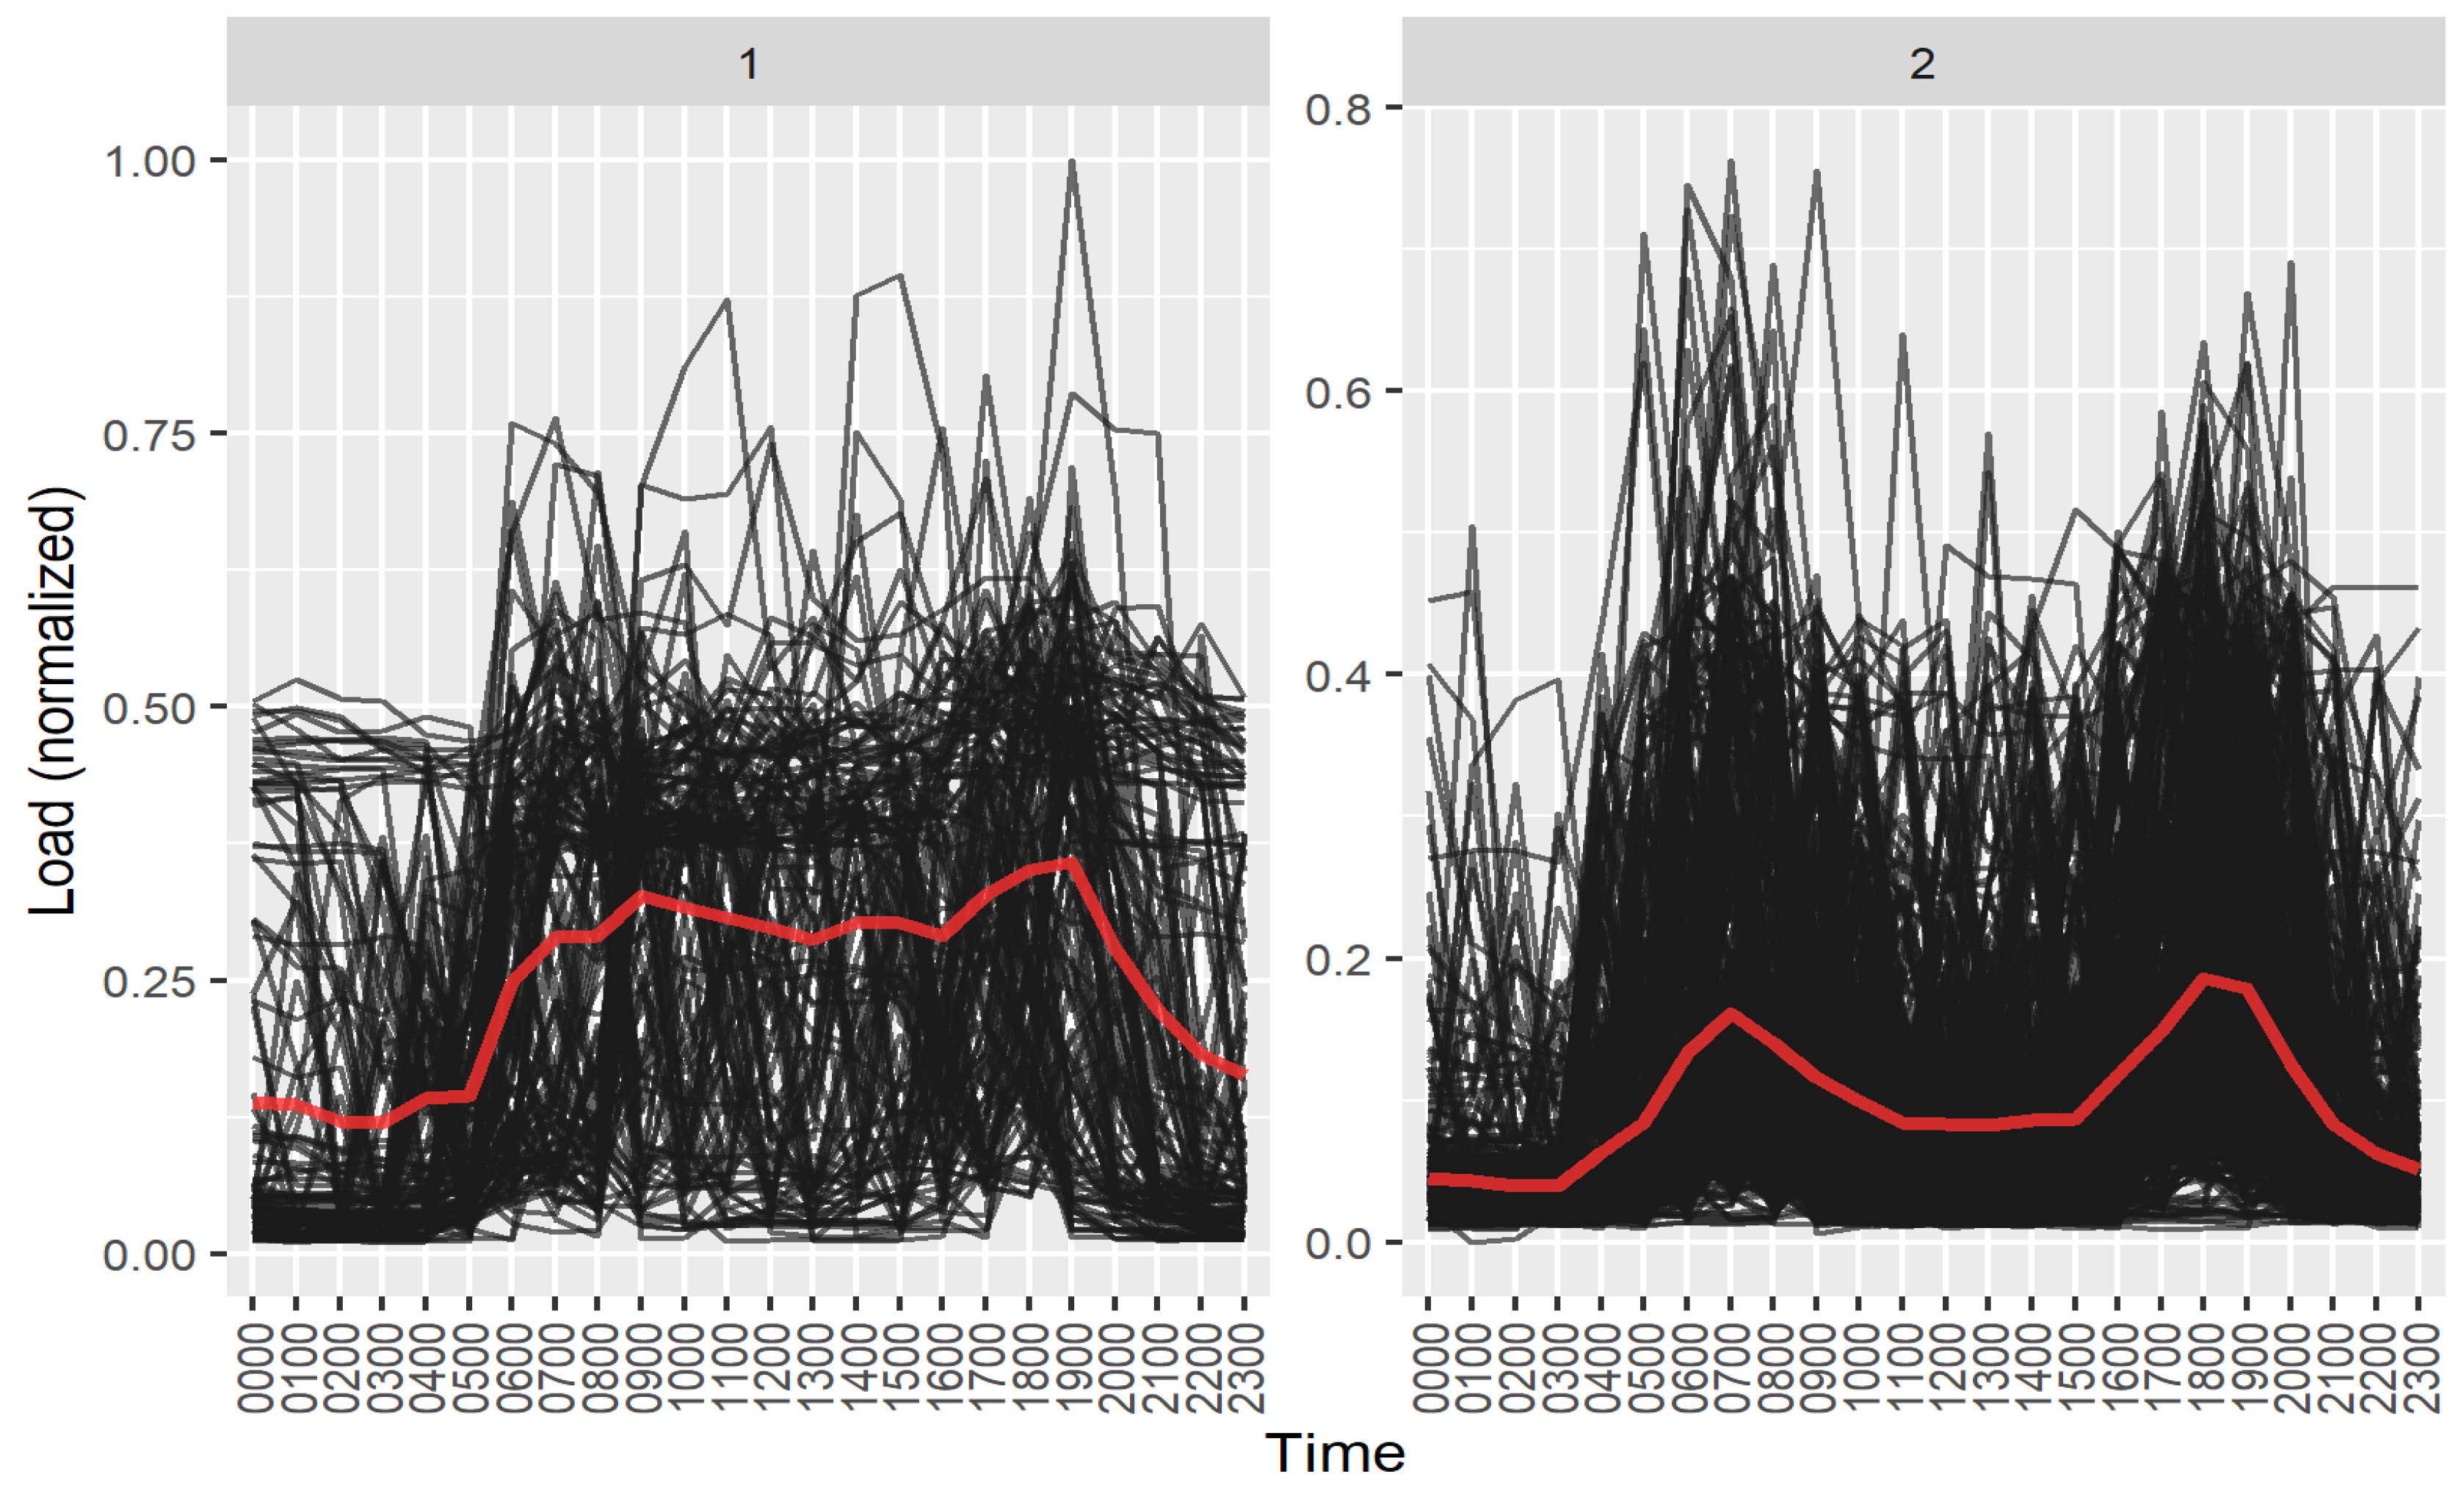
\includegraphics[width=0.8\textwidth]{figures/malatesta_hsop/malatesta_routinisedHousehold.jpg}
    \caption{K-Means resulting in Routinised Household Using all Year Energy Data \cite{MAL-HBP}}
    \label{fig:routinized_household}
\end{figure}

\begin{figure}
    \centering
    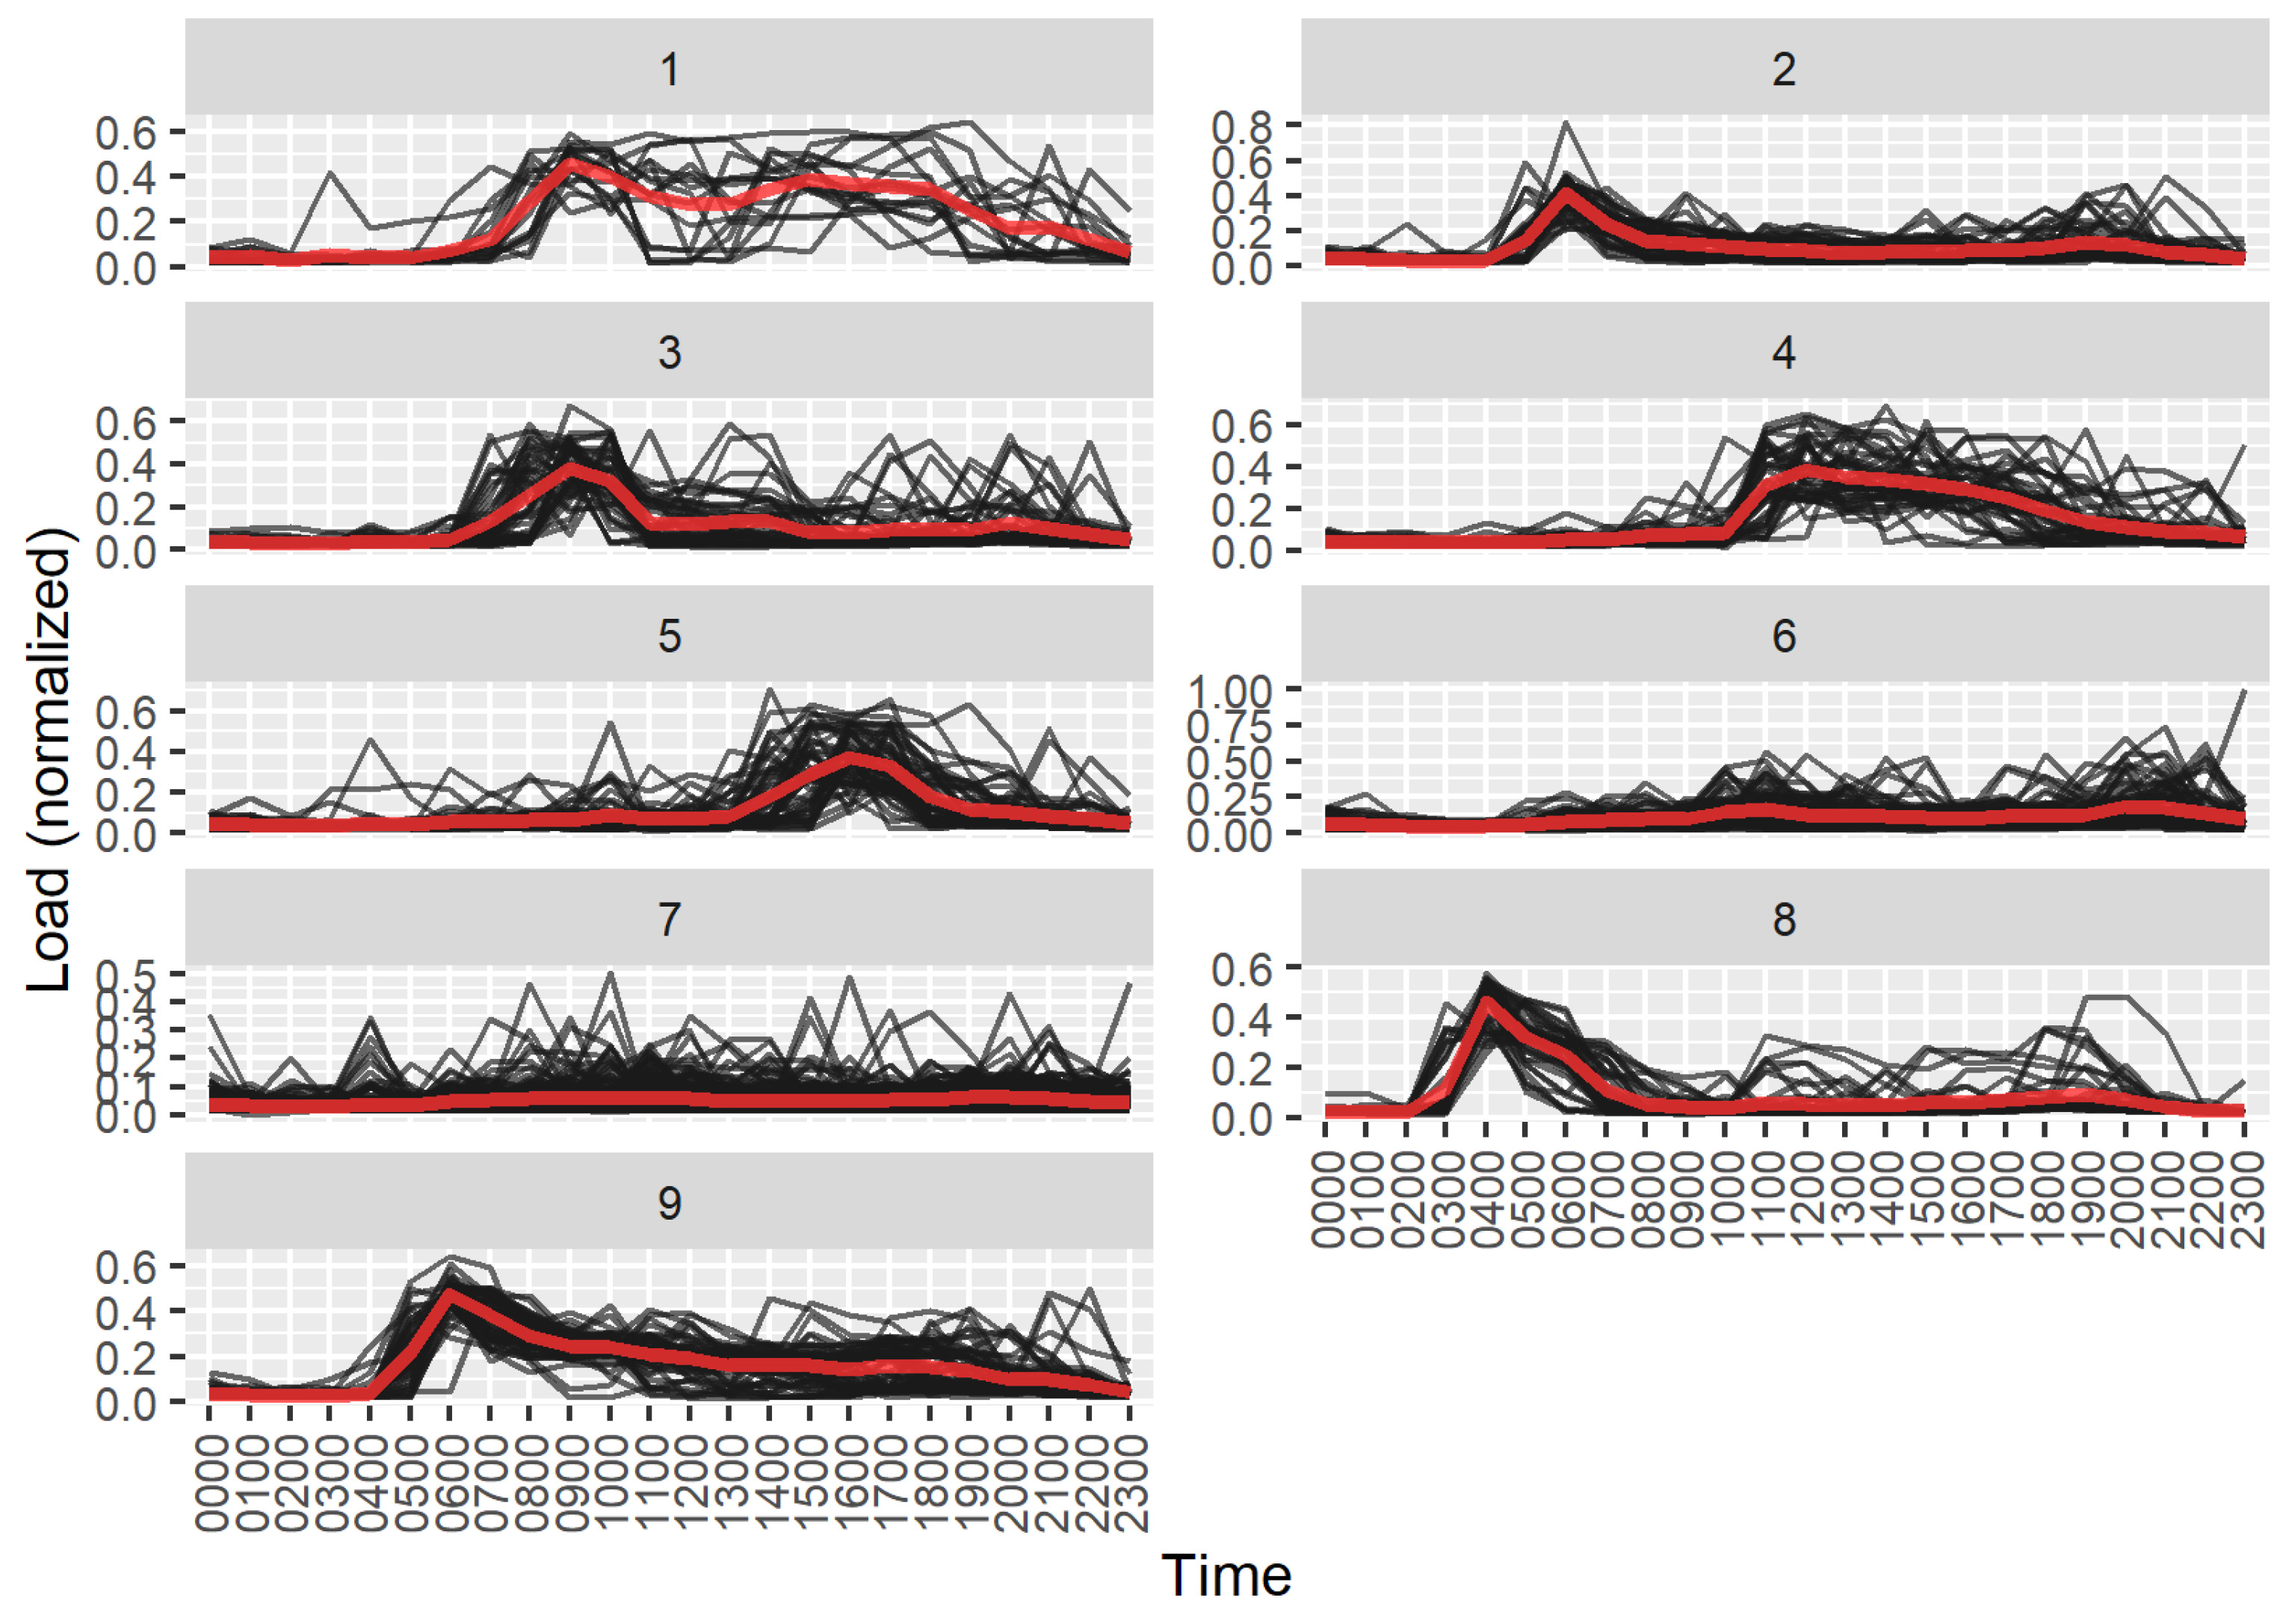
\includegraphics[width=0.8\textwidth]{figures/malatesta_hsop/malatesta_unroutinisedHousehold.jpg}
    \caption{K-Means resulting in Unroutinised Household Using all Year Energy Data \cite{MAL-HBP}}
    \label{fig:non_routinized_household}
\end{figure}

Variable lifestyles with different work commitments (e.g. working from home) or family structures (e.g. having children) alter the energy consumption of households \cite{KUR-HBP}.
If occupants are routinized, their behaviors are repetitive \cite{BRE-EWP}.
\section{Identifying and Differentiating Natural Disaster- and Electrical Fault-Impacted Load Profiles}
\label{sec:identifying_and_differentiating_natural_disaster_and_electrical_fault_impacted_load_profiles}
% One paragraph for each research question.
% Remember to include equations and figures, and cite everything!